\chapter[Регламентация конструкторских работ.\break Конструкторская документация]{Регламентация конструкторских работ.\\ Конструкторская документация}

\newthought{Конструирование} является составной частью проектирования и заключается в разработке конкретного варианта изделия на основе проведенных предварительных исследований. 

Организация процесса проектирования определяется степенью новизны и сложностью решаемой задачи. В зависимости от степени новизны различают:
\begin{itemize}
	\item частичную модернизацию существующего прибора (системы), приводящую к некоторому улучшению одного или нескольких показателей качества за счет изменения параметров, улучшения элементной базы, частичного изменения структуры;
	\item существенную модернизацию, приводящую к значительному улучшению основных показателей качества прибора (системы) за счет существенного изменения параметров и структурной схемы, приводящих к большим конструктивным изменениям;
	\item создание нового прибора (системы), предназначенного для решения известных или принципиально новых задач и основанного на новых принципах действия, использование которых позволяет резко улучшить основные показатели качества.
\end{itemize}

При создании новых ОЭП процессу собственно проектирования~-- опытно-конструкторским работам (ОКР)~-- обычно предшествуют научно-исследовательские работы (НИР).

Целью НИР является решение проблемных вопросов, позволяющее обосновать возможность и целесообразность дальнейшего проектирования, получить необходимую исходную информацию и тем самым предотвратить значительные затраты на проведение проектных работ в случае, когда поставленная задача не может быть решена предлагаемыми средствами.

В рамках НИР изучается состояние разработок по поставленной или родственным задачам. С этой целью анализируются все доступные источники информации, а также опыт промышленности. На основе выдвинутых теоретических положений разрабатываются макеты узлов и прибора в целом. После их изготовления и экспериментальных исследований дается заключение о возможности создания промышленного образца прибора и формулируются рекомендации по проведению ОКР.

Последовательность разработки и изготовления промышленных изделий в настоящее время регламентируется группой государственных стандартов, входящих в Единую систему конструкторской документации (ЕСКД).

ЕСКД устанавливает единый порядок разработки, выполнения, оформления, согласования, внесения изменений, учета и хранения конструкторской документации.

В соответствии с действующим стандартом (ГОСТ~2.103–68) проектирование ОЭП можно представить в виде последовательности этапов, в процессе которых разрабатывают ТЗ, техническое предложение, эскизный, технический и рабочий проекты (рис.~\ref{pic:etapi}).

\begin{figure}[h!]
	\begin{center}
		
\includegraphics[width=0.45\linewidth]{etapi.png}
		\caption{Этапы проектирования}
		\label{pic:etapi}
	\end{center}
\end{figure}

Перечисленные этапы позволяют обеспечить изготовление опытного образца, который затем испытывается. 
По результатам испытаний в конструкцию вносятся необходимые изменения и уточнения, и после окончательных испытаний дается заключение о возможности изготовления установочной серии приборов. 
В зависимости от потребностей в данном приборе в дальнейшем осуществляется переход к мелкосерийному, серийному или массовому производству.

Следует отметить, что в зависимости от назначения и области применения прибора (системы), необходимых сроков разработки, а также в связи с внедрением современных методов системного и автоматизированного проектирования последовательность и содержание этапов могут изменяться. 
Например, если на этапе технического предложения получено полное представление о схемном и конструктивном решении прибора, этап эскизного проектирования может не выполняться, и разработчик сразу переходит к техническому проектированию. 
Для ускорения процесса проектирования иногда могут быть совмещены технический и рабочий проекты. 
Однако при создании большинства современных приборов указанная последовательность проектирования выдерживается.

\section{Техническое задание}
Проектирование любого промышленного изделия, в том числе и ОЭП, ведется на основании технического задания (ТЗ).

\noindent
\textsc{Техническое задание} --- это документ, который устанавливает назначение и область применения, технические, качественные и технико-экономические требования, а также определяет необходимые стадии разработки конструкторской документации и ее состав.

ТЗ составляется организацией-заказчиком при возможном участии организации-разработчика с привлечением других заинтересованных организаций. После утверждения и согласования ТЗ принимается к выполнению.

ТЗ на проектирование ОЭП обычно состоит из нескольких разделов.

Вводная часть ТЗ содержит основание для проведения ОКР. В следующем разделе указываются назначение и область применения изделия. Далее излагаются технические требования, предъявляемые к изделию.

К техническим требованиям относятся:
\begin{itemize}
	\item диапазон и точность измерений; 
	\item дальность действия;
	\item чувствительность или разрешающая способность; выходные параметры прибора, обеспечивающие его стыковку с другими системами (если данный ОЭП входит в состав какого-либо комплекса), либо форма представления информации об измеряемой величине (напряжение, код, вход в ЭВМ), если прибор решает самостоятельную задачу. При этом могут предъявляться требования к крутизне и диапазону линейности выходных характеристик прибора;
	\item спектральный диапазон работы, параметры и характеристики излучения исследуемого или измеряемого объекта;
	\item конструктивные требования к схемам и узлам прибора (кинематическим, электрическим, оптическим);
	\item габаритные размеры и масса прибора или отдельных его частей;
	\item требования по видам потребляемой энергии и мощности потребления;
	\item требования к тепловыделению прибора, а при необходимости охлаждения -- параметры системы охлаждения;
	\item требования по соответствию параметров прибора или его конструктивного исполнения определенным ГОСТам, ОСТам и другим нормативным документам.
\end{itemize}


В соответствующем разделе дается полная характеристика условий работы изделия, среди которых можно назвать:
\begin{itemize}
	\item характер помех, определяемый либо конкретным указанием их энергетических, спектральных и пространственных характеристик, либо указаниями общего порядка (например, облачное небо, звездный фон, вид ландшафта);
	\item параметры или характеристики, определяющие прохождение излучения для ОЭП, работающих в полевых или других неблагоприятных условиях (например, данные о среде распространения и ее параметрах, метеорологической дальности видимости, наличии задымленности);
	\item характер размещения прибора и в связи с этим различные динамические факторы условий эксплуатации (вибрация, перегрузки, ударные воздействия);
	\item динамические свойства исследуемого объекта -- частота колебаний, перемещения, распределение параметров по гармоническим составляющим и др.;
	\item метеорологические факторы -- температурный диапазон, влажность, давление, воздействие осадков, пыли, морского тумана, солнечной радиации;
	\item требования к защите прибора от воздействия полей и излучений;
	\item условия хранения и транспортирования;
	\item диапазон возможных отклонений параметров системы энергопитания.
\end{itemize}

В специальном разделе ТЗ излагаются требования по надежности и работоспособности, в том числе:
\begin{itemize}
	\item гарантийный срок службы прибора при обусловленных ТЗ условиях эксплуатации;
	\item периодичность проверок, аттестаций и профилактического ремонта;
	\item режимы работы, в частности время непрерывной работы, периодичность включения;
	\item время готовности прибора к работе от момента включения электропитания;
	\item требования к надежности работы в течение определенного времени с требуемой вероятностью безотказной работы;
	\item требования к жесткости, надежности крепления элементов и узлов, системе амортизации;
	\item требования к безопасности работы с прибором.
\end{itemize}

В ТЗ включаются также разделы, в которых излагаются требования по охране труда, технической эстетике, технологичности, отражаются технико-экономические показатели, специальные требования, учитывающие специфику построения, применения и изготовления прибора.

В одном из заключительных разделов ТЗ отражаются этапы создания прибора и состав технической документации, разрабатываемой на каждом этапе и ОКР в целом, другие аспекты проектирования, имеющие принципиальное значение. После оформления и утверждения ТЗ приступают непосредственно к проектным работам.

Следует отметить, что в процессе выполнения ОКР техническое задание может уточняться по взаимному согласованию заинтересованных сторон в случаях, если будет доказана необоснованность каких-либо требований, показана принципиальная невозможность обеспечения некоторых свойств.

\section{Техническое предложение}

\noindent
ГОСТ~2.118–2013: \textsc{техническое предложение} разрабатывают в целях выявления дополнительных или уточненных технических и эксплуатационных требований к прибору, которые не были отражены в ТЗ и для обоснования которых целесообразно выполнить предварительную конструкторскую проработку и анализ различных вариантов решения.

Наиболее типичными видами работ, проводимых на этапе технического предложения, являются:
\begin{itemize}
	\item научно-технический поиск в целях подбора и изучения всех доступных  материалов по проектируемому изделию;
	\item анализ полученной информации и выявление положений, позволяющих наметить варианты решения поставленной в ТЗ задачи;
	\item установление возможных вариантов схемы и конструкции прибора;
	\item сравнительная, оценка выявленных вариантов по различным показателям, определенным ТЗ;
	\item проверка вариантов на патентную чистоту и конкурентоспособность, оформление заявок на изобретение;
	\item проверка соответствия возможных вариантов требованиям стандартизации, унификации, техники безопасности, эргономики;
	\item предварительная оценка технологичности конструкции прибора.
\end{itemize}

В процессе выполнения указанных работ на данном этапе могут быть проведены различные расчеты, а также экспериментальные исследования с использованием математических моделей и макетов. Для изготовления макетов должна быть разработана конструкторская документация.

Результатом работ на данном этапе должно быть ТЗ, сформулированное с учетом положений, выявленных в процессе теоретических и экспериментальных исследований, а также конструкторская документация (КД), дающая обобщенное представление о выявленных технических решениях.

На рассматриваемом этапе наряду с учетом конструктивных и эксплуатационных особенностей существующих изделий аналогичного назначения необходимо иметь в виду тенденции и перспективы развития отечественной и зарубежной техники в данной области.

Следует уже при проведении данного этапа проектирования стремиться к выбору оптимального варианта прибора, так как это позволит избежать ненужных затрат на последующих этапах и ускорит проектирование. В случае невозможности такого выбора необходимо установить дополнительные требования к последующим этапам.

Конструкторская документация, выпускаемая на этапе технического предложения, включает обобщенные схемы ОЭП, упрощенные чертежи общего вида, габаритный чертеж, ведомость технического предложения, пояснительную записку, патентный формуляр.

Пояснительная записка в соответствии с действующим стандартом (ГОСТ~2.106-68) в общем случае должна включать следующие разделы:
\begin{itemize}
	\item введение (с указанием документов, на основании которых выполняется проектирование);
	\item назначение и область применения  прибора;
	\item технические характеристики прибора;
	\item описание и обоснование выбранной конструкции;
	\item расчеты, подтверждающие работоспособность и надежность выбранного конструктивного решения;
	\item описание организации работ с применением разрабатываемого прибора;
	\item ожидаемые технико-экономические показатели;
	\item уровень оценки по показателям стандартизации, унификации, патентной чистоты.
\end{itemize}

Указанная структура пояснительной записки применима к любому этапу проектирования. При этом в зависимости от особенностей изделия и характера решаемых на том или ином этапе проектирования задач возможно объединение, исключение или введение новых разделов.

Пояснительная записка должна быть оформлена в соответствии с действующим стандартом~(ГОСТ~2.105-79). Чертежи и схемы выполняются с максимальными упрощениями, предусмотренными ЕСКД.

После рассмотрения и утверждения технического предложения его материалы служат основой для проведения последующих этапов проектирования.

\section{Эскизное проектирование}

\noindent
ГОСТ 2.119–2013: \textsc{эскизный проект} является проектной стадией разработки КД и его следует разрабатывать в соответствии с ТЗ с целью установления принципиальных конструктивных решений, дающих общее представление об устройстве, принципах работы и габаритных размерах разрабатываемого изделия, а также данных, определяющих основные параметры, когда это целесообразно сделать до разработки ТП или рабочей КД.

При выполнении эскизного проекта проводят:
\begin{itemize}
	\item проработку возможных вариантов схемного и конструктивного решений прибора;
	\item расчетное обоснование их ожидаемых технических характеристик;
	\item оценку возможности реализации полученных вариантов на основе освоенной промышленностью номенклатуры материалов и комплектующих изделий;
	\item оценку технологичности конструкции и возможностей изготовления прибора в условиях конкретной производственной базы;
	\item проверку принятых технических решений на патентную чистоту и оформление заявок на изобретения в случае положительных результатов патентных исследований;
	\item проверку решений на соответствие требованиям техники безопасности, стандартизации и унификации;
	\item проработку художественно-конструкторских вопросов, оценку прибора по показателям эргономики.
\end{itemize}

С учетом полученных результатов перечисленных работ выполняется сравнительная оценка вариантов по установленным ТЗ показателям и обобщенным критериям оценки качества ОЭП и выбирается оптимальный вариант прибора.

На этапе эскизного проектирования на основе принятых принципиальных решений большое внимание уделяется выявлению на основе принятых принципиальных решений новых изделий и материалов, которые планируется разработать и изготовить другими предприятиями (например, источников и приемников излучения, электромеханических элементов, шарико-подшипников, конструкционных и других материалов). На этом этапе должны быть составлены технические требования к таким изделиям и материалам и определен круг их возможных разработчиков.

С целью более обоснованного выбора оптимального варианта прибора может быть проведено макетирование его отдельных узлов или прибора в целом с последующим исследованием макетов.

Важное значение при эскизном проектировании имеет оценка метрологического обеспечения будущего серийного или массового производства прибора. Это прежде всего относится к прецизионным приборам, поскольку для оценки их точностных возможностей может потребоваться уникальное оборудование (стенды). В некоторых случаях для создания такого оборудования необходимы значительные усилия, вплоть до проведения самостоятельных НИР и ОКР, на выполнение которых должно быть выдано соответствующее ТЗ.

Иногда уже на этапе эскизного проектирования предварительно решают вопросы упаковки и транспортирования, например при проектировании крупногабаритных изделий или изделий, для которых требуется специальная упаковка или средства транспортирования.

На этапе эскизного проектирования при необходимости выполняют и другие работы. В то же время обычно не повторяют работы, проведенные на этапе технического предложения, если они не могут дать дополнительных данных. В этом случае результаты ранее проведенных работ отражаются в пояснительной записке.

\textsc{Конструкторская документация эскизного проекта} включает:
\begin{itemize}
	\item основные схемы прибора;
	\item чертеж общего вида;
	\item чертежи основных сборочных единиц;
	\item габаритный чертеж;
	\item ведомость эскизного проекта;
	\item пояснительную записку.
\end{itemize} 

\textsc{Схемы прибора} разрабатывают на основе выбранного принципа его работы и проведенных расчетов. 
Как правило, выполняются функциональные или принципиальные схемы следующих видов: оптические, электрические, кинематические. 
Схемы должны давать полное представление о принципе работы прибора, взаимосвязях всех его узлов и элементов.

\textsc{Чертеж общего вида}\marginnote{\allcaps{ЧЕРТЁЖ ОБЩЕГО ВИДА}} выполняется с упрощениями, предусмотренными ЕСКД, и должен давать представление о компоновке прибора, взаимодействии его основных составных частей. 
При эскизном проектировании на чертеже общего вида часто используют контурное изображение заимствованных сборочных единиц, покупных и других комплектующих изделий (объективов, электродвигателей, подшипников).

\textsc{Габаритный чертеж}\marginnote{\allcaps{ГАБАРИТНЫЙ ЧЕРТЁЖ}} представляет собой контурное (упрощенное) изображение прибора с габаритными, установочными и присоединительными размерами и является необходимым конструкторским документом, если прибор входит в состав каких- либо сложных систем, комплексов или должен быть установлен (смонтирован) на специальных основаниях. 
Габаритный чертеж разрабатывается по согласованию со смежными организациями и окончательно уточняется на этапе технического проекта.

\textsc{Пояснительная записка}\marginnote{\allcaps{ПОЯСНИТЕЛЬНАЯ\break ЗАПИСКА}} эскизного проекта выполняется с учетом следующих требований к содержанию разделов.

При изложении технической характеристики наряду с указанием свойств прибора приводятся сведения об отклонениях или соответствии требованиям ТЗ и сравнительные данные отечественных и зарубежных аналогов.

Раздел <<Описание и обоснование выбранной конструкции>> наряду с изложением принятых схемных и конструктивных решений может содержать сведения о макетах прибора, методике и результатах их испытаний, сведения о технологичности, дополнительные результаты патентных исследований, сведения о вновь разрабатываемых материалах и комплектующих изделиях.

Пояснительная записка эскизного проекта должна содержать все необходимые расчеты ОЭП, подтверждающие возможность его реализации. При большом объеме расчетов они могут быть оформлены в виде отдельного документа. При этом в пояснительной записке приводятся только результаты расчетов.
К числу наиболее важных относятся следующие виды расчетов ОЭП: энергетический (светотехнический); оптической системы (габаритный, аберрационный); электронного тракта; точности. В зависимости от принципа работы ОЭП проводят и другие расчеты, часто имеющие принципиальное значение: кинематический, динамический, надежности, прочности и жесткости, температурных режимов.

Приложение к пояснительной записке может включать сведения по стандартизации и унификации, материалы художественно-конструкторской проработки, в частности результаты эргономического анализа, требования по технике безопасности и другие материалы, представляющие интерес для всесторонней характеристики проектируемого прибора.

Эскизный проект рассматривается заинтересованными организациями и защищается в установленном порядке. 
Выявленные в результате рассмотрения и защиты замечания либо устраняются, либо по ним намечаются мероприятия для последующих этапов проектирования, после чего протокол о защите утверждается.

\section{Техническое проектирование}

\noindent
ГОСТ 2.120–2013: \textsc{технический проект} является проектной стадией разработки КД и его следует разрабатывать в соответствии с ТЗ с целью выявления окончательных технических решений, дающих  полное представление об устройстве разрабатываемого изделия, и исходных данных для разработки рабочей КД, когда это целесообразно сделать до разработки рабочей КД. 

Основными видами работ являются:
\begin{itemize}
	\item детальная разработка конструкции всего прибора и его составных частей;
	\item разработка принципиальных схем, на основе которых могут быть выполнены монтажные схемы, схемы соединений, осуществлены сборка и настройка оптических и электронных блоков;
	\item окончательное оформление заявок и ТЗ на изготовление новых изделий и материалов;
	\item выявление номенклатуры покупных изделий и согласование их применения;
	\item окончательное согласование габаритных, установочных и присоединительных размеров, мест подключения разъемов с заказчиком и основными потребителями;
	\item анализ конструкции прибора, его узлов и отдельных наиболее сложных и ответственных деталей на технологичность и определение на основе этого анализа возможности использования имеющегося на предприятии оборудования, необходимости приобретения или создания нового технологического оборудования и спецоснастки;
	\item окончательное решение вопросов метрологического обеспечения по выбору средств измерений и методов контроля метрологических характеристик приборов;
	\item проверка принятых технических решений на соответствие требованиям стандартизации, унификации, техники безопасности;
	\item проверка приборов на патентную чистоту, оформление заявок на изобретения;
	\item окончательное решение вопросов транспортирования, хранения и монтажа на месте эксплуатации;
	\item оценка эксплуатационных характеристик приборов, в частности взаимозаменяемости, удобства обслуживания, ремонтопригодности, устойчивости к воздействию факторов внешней среды, возможности быстрого устранения отказов, контроля качества работы, обеспеченности средствами контроля технического состояния и др.
\end{itemize}

Как правило, разработка технического проекта сопровождается большим объемом макетирования. Макеты создаются в целях проверки конструктивных и схемных решений прибора, а также для подтверждения окончательно принятых решений. 

При этом наряду с функционирующими макетами целесообразно делать макеты-муляжи (например, из дерева), на которых можно проверить удобство обслуживания и расположения элементов, т. е. отработать эргономические и художественно-конструкторские показатели.

Выполняемые при техническом проектировании расчеты служат для окончательного установления свойств прибора, выработки требований к узлам и отдельным ответственным деталям. На этом этапе проектирования уточняются такие показатели, как инструментальная составляющая суммарной погрешности, которая может быть выявлена только на основе окончательно принятых конструктивных решений. 

Особое внимание уделяется подбору необходимого оборудования для лабораторных испытаний будущих приборов.

В результате технического проектирования обычно выпускается следующая \textsc{конструкторская документация}: 
\begin{itemize}
	\item чертежи общего вида;
	\item чертежи сборочных единиц;
	\item габаритный чертеж;
	\item чертежи всех схем;
	\item ведомость технического проекта;
	\item пояснительная записка;
	\item приложение к пояснительной записке;
	\item ведомость покупных изделий;
	\item ведомость согласования применения покупных изделий;
	\item патентный формуляр;
	\item карта технического уровня.
\end{itemize}

Пояснительная записка технического проекта включает те же разделы, что и записка к эскизному проекту. Однако в ней особое внимание уделяется обоснованию и описанию конструктивных особенностей прибора, принципов его функционирования, В нее включаются расчеты, выполненные по ходу технического проекта, Существенно расширяется раздел, посвященный описанию организации работ с прибором на месте эксплуатации. В этом разделе даются сведения о приемах и способах работы с прибором, транспортировании, монтаже и хранении, количестве и квалификации обслуживающего персонала.

В приложении к пояснительной записке могут быть приведены расчеты, материалы ху\-до\-жест\-вен\-но-конструкторской проработки.

Технический проект подлежит защите и утверждению заказчиком.

\section{Рабочее проектирование}
Рабочий проект выполняется с целью создания и отработки полного комплекта конструкторской документации ОЭП, достаточной для изготовления опытного образца прибора. Рабочее проектирование может выполняться как самостоятельный этап, но иногда для ускорения процесса проектирования его начинают на этапе технического проекта (технорабочий проект). Этап рабочего проектирования характеризуется тесным взаимодействием конструкторских и технологических подразделений предприятия.

Основными видами работ на этом этапе являются:
\begin{itemize}
	\item детальная разработка конструкции прибора и его узлов с указанием технологических требований к сборке и юстировке;
	\item доведение всех схем до рабочего состояния (выполняются монтажные схемы, на оптических схемах приводятся требования по юстировке);
	\item составление спецификаций и сводных ведомостей покупных и стандартных изделий и деталей, марок и сортаментов применяемых материалов;
	\item разработка ведомостей и чертежей согласования применения готовых изделий;
	\item согласование методик юстировки, настройки, монтажа, испытаний;
	\item составление технического описания, технических условий, инструкций по эксплуатации, формуляра, технического паспорта;
	\item составление ведомости запасного инструмента и принадлежностей (ЗИП);
	\item разработка технологических процессов изготовления наиболее сложных и ответственных деталей.
\end{itemize}

\newthought{Рабочие чертежи}\marginnote{\allcaps{РАБОЧИЕ ЧЕРТЕЖИ}} должны обеспечивать возможность оптимального применения стандартных, покупных и освоенных ранее изделий, рационально ограниченную номенклатуру материалов, покрытий, размеров, резьб, допусков, необходимую степень взаимозаменяемости, экономичные способы изготовления, максимальное удобство при эксплуатации.

В процессе рабочего проектирования выполняются контрольно-сборочные чертежи узлов и прибора в целом для выявления ошибок в рабочих чертежах деталей до их изготовления и сборки. Контрольно-сборочный чертеж вычерчивают по рабочим чертежам деталей путем считывания всех необходимых размеров, проверки правильности простановки допусков на сопрягаемые детали и тщательного переноса размеров в соответствии с необходимым масштабом на поле чертежа.

Все выявленные ошибки и неточности рабочих чертежей устраняются, после чего чертежи проходят нормоконтроль по действующему стандарту (ГОСТ~2.111-68), технологический контроль и утверждаются.

Рабочие чертежи деталей и сборочные чертежи являются основной документацией, руководствуясь которой можно осуществить изготовление \textsc{опытного образца} прибора. Дополнением к ним являются технические условия, содержащие все отсутствующие в чертежах, но необходимые для изготовления и отладки технические требования, а также требования на приемку и испытания.

Технические условия составляют в соответствии с ГОСТ~2.114-70 на основе ТЗ, чертежей и документации технического проекта.
Составление методики юстировки и настройки должно быть увязано с выпуском рабочих чертежей контрольно-юстировочной аппаратуры.

После подготовки и утверждения всей необходимой документации опытное производство предприятия изготавливает опытный образец или партию приборов. Конструкторские подразделения предприятия осуществляют наблюдение за ходом изготовления и оказывают необходимую помощь производству. Возникающие в процессе изготовления замечания к документации исправляются.

Изготовленные опытным производством образцы приборов передаются на всесторонние испытания. При проведении предварительных испытаний проверяют правильность функционирования, соответствие приборов техническим условиям и техническому паспорту. Эти испытания могут проводиться как в условиях заводской испытательной лаборатории (на соответствующих стендах), так и в условиях предполагаемой эксплуатации. Если изготовленные приборы прошли предварительные испытания, их передают на государственные испытания для полной проверки опытного образца прибора на соответствие ТЗ и техническим условиям. Так же, как и предварительные, государственные испытания могут проводиться в лабораторных и полевых условиях.

Государственные испытания осуществляются под руководством государственной комиссии, состоящей из специалистов отраслевых НИИ, представителей заказчика и предприятия-раз\-ра\-бот\-чи\-ка. Испытания регламентируются специальной программой. Государственным испытаниям подвергаются приборы, прошедшие предварительные испытания и снабженные всей необходимой технической документацией, что подтверждается соответствующим актом.

В процессе государственных испытаний фиксируются все замечания. Если они легко устранимы, то испытания продолжаются; если носят принципиальный характер, то опытные образцы и документация возвращаются на доработку, после которой вновь представляются на испытания.

По окончании испытаний составляется акт, где дается заключение о соответствии прибора ТЗ и о возможности его запуска в серийное или массовое производство, а также приводятся замеченные недостатки, которые должны быть устранены в процессе подготовки прибора к следующему этапу производства.

Перед серийным производством обеспечивается технологическая подготовка производства, заключающаяся в проектировании технологического процесса изготовления деталей и сборки, конструировании и изготовлении технологической оснастки, разработке методики контроля технических характеристик прибора и проектировании соответствующей контрольно-юс\-ти\-ро\-воч\-ной аппаратуры.

По окончании этапа технологической подготовки производства может быть изготовлена установочная партия приборов, на которой окончательно отрабатываются конструкторская документация и технологический процесс, а также проверяются наличие требуемых технологической оснастки и контрольно-юстировочной аппаратуры и их возможности. При соответствии установочной партии приборов и технической документации предъявляемым требованиям приборы запускаются в серийное производство.

\section{Конструкторская документация}
На всех этапах жизненного цикла (разработка -- производство -- эксплуатация) ОЭП сопровождает техническая документация (ТД). Состав этой документации и ее содержание регламентируется Государственными стандартами. В настоящее время в стране действует большое количество стандартов, которые сгруппированы по направлениям жизненного цикла изделий в следующие комплексы:
\begin{itemize}
	\item единая система конструкторской документации (ЕСКД);
	\item единая система технологической документации (ЕСТД);
	\item единая система программной документации (ЕСПД);
	\item единая система технологической подготовки производства (ЕСТПП);
	\item единая система защиты изделий и материалов от коррозии, старения и биоповреждений (ЕСЗКС).
\end{itemize}

Государственные стандарты, входящие в ЕСКД, устанавливают взаимосвязанные единые правила и положения по порядку разработки, оформления и обращения конструкторской документации на изделия, разрабатываемые и выпускаемые предприятиями всех отраслей промышленности.

\textsc{Конструкторские документы (КД)}\marginnote{\allcaps{КОНСТРУКТОРСКИЕ\break ДОКУМЕНТЫ}} --- графические и текстовые документы, в отдельности или в совокупности определяющие состав и устройство изделия и содержащие необходимые данные для его разработки и изготовления, контроля, приемки, эксплуатации, ремонта, утилизации.

Стандартам ЕСКД присваивают обозначения по классификационному принципу. Номер стандарта составляется из цифры, присвоенной классу стандартов ЕСКД, одной цифры после точки, обозначающей классификационную группу стандартов в соответствии с таблицей 1, числа, определяющего порядковый номер стандарта в данной группе, и двузначной цифры (после тире), указывающей год регистрации стандарта. Например, обозначение стандарта ЕСКД <<ЕСКД. Схемы. Виды и типы. Общие требования к выполнению>> имеет вид:
\begin{description}
	\item[ГОСТ 2.701-84]:
	\item[ГОСТ] -- категория нормативно-технического документа (государственный стандарт);
	\item[2] -- класс (стандарты ЕСКД);
	\item[7] -- классификационная группа стандартов; 
	\item[01] -- порядковый номер стандарта в группе; 
	\item[84] -- год регистрации стандарта.
\end{description}

Разработка и изготовление любого ОЭП связаны с выпуском конструкторской документации, которая полностью и однозначно определяют все необходимые и достаточные данные для изготовления, настройки и юстировки, приемки, эксплуатации и ремонта как всего прибора в целом, так и его составных частей.

\begin{table*}[ht]
	\fontfamily{ppl}\selectfont
	\begin{tabular}{cl} \hline 
		\toprule
		Шифр группы & Содержание стандартов в группе \\
		\midrule
		0 & Общие положения \\
		1 & Основные положения \\
		2 & Классификация и обозначение изделий в КД \\
		3 & Общие правила выполнения чертежей \\
		4 & Правила выполнения чертежей изделий машиностроения и приборостроения \\
		5 & Правила обращения КД (учет, хранение, дублирование, внесение изменений) \\
		6 & Правила выполнения эксплуатационной и ремонтной документации \\
		7 & Правила выполнения схем \\
		8 & Правила выполнения документов строительных, судостроительных и горных дел \\
		9 & Прочие стандарты \\
		\bottomrule \\
	\end{tabular}
	\label{tab:standart}
	\caption{Перечень классификационных групп стандартов ЕСКД}
\end{table*}

Согласно действующему стандарту (ГОСТ~2.102-68) к конструкторской документации относятся следующие графические и текстовые документы:
\begin{itemize}
	\item чертеж детали, содержащий изображение детали и другие данные, необходимые для ее изготовления и контроля;
	\item сборочный чертеж (СБ), содержащий изображение сборочной единицы и другие данные, необходимые для ее сборки и контроля;
	\item чертеж общего вида (ВО), определяющий конструкцию прибора, взаимодействие его основных составных частей, поясняющий принцип работы изделия, включая форму деталей и характерные размеры, которые облегчают уяснение формы элементов деталей, содержащий предельные отклонения сопрягаемых поверхностей и сопровождаемый техническими требованиями к прибору;
	\item теоретический чертеж (ТЧ), определяющий геометрическую форму прибора и координаты расположения составных частей;
	\item габаритный чертеж (ГЧ), представляющий собой контурное (упрощенное) изображение прибора с габаритными, установочными и присоединительными размерами;
	\item монтажный чертеж (МЧ) -- упрощенное изображение прибора с данными, необходимыми для его установки на месте эксплуатации;
	\item схемы по действующему стандарту (ГОСТ 2.701-84), на которых показаны в виде условных изображений или обозначений составные части изделия и связи между ними;
	\item спецификация -- документ, определяющий состав сборочной единицы, комплекса или комплекта. Спецификация в общем случае состоит из разделов: документация, комплексы, сборочные единицы, детали, стандартные изделия, прочие изделия, материалы, комплекты. Требования к выполнению спецификаций регламентирует действующий стандарт (ГОСТ 2.108-68);
	\item ведомости спецификаций (ВС), ссылочных документов(ВД), покупных изделий (ВП), согласования применения изделий (ВИ), держателей подлинников (ДП), технического предложения (ПТ), эскизного проекта (ЭП), технического проекта (ТП);
	\item пояснительная записка (ПЗ) содержит описание прибора и принципа его действия, а также обоснование принятых при разработке прибора технических и технико-экономических решений;
	\item технические условия (ТУ) содержат требования к прибору и его составным частям и деталям и обычно включают следующие разделы: вводную часть с указанием назначения, области применения прибора и условий его эксплуатации; состав комплекта прибора; технические требования к материалам, отдельным деталям, сборочным единицам и прибору в целом; требования к покрытиям и окраске; методы контроля технических характеристик, порядок приемки, поверок и испытаний; требования к транспортированию и хранению, смазыванию, упаковке; порядок маркировки; указания о гарантийных обязательствах изготовителя;
	\item программа и методика испытаний (ПМ);
	\item патентный формуляр (ПФ);
	\item карта технического уровня и качества изделия (КУ), характеризующая уровень качества прибора, соответствие его технических и экономических показателей достижениям науки и техники и потребностям народного хозяйства;
	\item таблицы (ТБ);
	\item расчеты (РР);
	\item инструкции (И), представляющие собой документы, используемые при изготовлении прибора (сборке, регулировании, контроле, приемке).
\end{itemize}

Помимо конструкторских документов в соответствии с ГОСТ~2.601-68 разрабатывается комплект эксплуатационных документов, в том числе:
\begin{itemize}
	\item техническое описание (ТО), дающее общее представление о приборе, его технических характеристиках, принципе его работы и устройстве, комплектации и другие сведения;
	\item инструкция по эксплуатации (ИЭ), которая может быть частью технического описания, но может быть и самостоятельным документом. В инструкции приводятся методика работы с прибором и его поверки, правила монтажа, подготовки прибора к работе, обращения с прибором, разборки, чистки, смазывания, транспортирования, а также указания по технике безопасности;
	\item технический паспорт (ПС) и формуляр (ФО) -- документы, сопровождающие прибор в процессе эксплуатации. Технический паспорт включает основные номинальные технические характеристики прибора, результаты исследования технических характеристик, состав комплекта, свидетельство о приемке, положения о гарантиях и сведения о рекламациях, номер прибора и номера комплектующих изделий. В формуляре наряду с основными сведениями, приведенными в паспорте прибора, даются сведения о режиме работы, учете времени эксплуатации, отметки о текущем состоянии прибора, его техобслуживании и ремонте;
	\item ведомость ЗИП (ЗИ) устанавливает номенклатуру, назначение и количество запасных частей, инструментов, принадлежностей и материалов, необходимых при эксплуатации и ремонте прибора;
	\item ведомость эксплуатационных документов (ЭД).
\end{itemize}

Состав ремонтных документов определяется ГОСТ~2.602-68. Эти документы предусматривают технически возможное и экономически целесообразное восстановление технических параметров прибора при эксплуатации на различных стадиях.

Важное место в конструкторской документации ОЭП принадлежит схемам. В соответствии с ГОСТ~2.701-84 виды схем обозначаются буквами, а их типы -- цифрами. В оптико-электронном приборостроении используются в основном схемы следующих видов:
\begin{description}
	\item[Э] -- электрические;
	\item[К] -- кинематические;
	\item[Л] -- оптические;
	\item[С] -- комбинированные.
\end{description}

Схемы в зависимости от их типа имеют следующие обозначения:
\begin{description}
	\item[1] -- структурные;
	\item[2] -- функциональные;
	\item[3] -- принципиальные;
	\item[4] -- соединений;
	\item[5] -- подключения;
	\item[6] -- общие;
	\item[7] -- расположения.
\end{description}

Например, схема электрическая функциональная имеет шифр Э2.

Специфическими конструкторскими документами ОЭП являются комбинированная функциональная и оптическая принципиальная схемы.

Функциональная комбинированная схема иллюстрирует процессы преобразования сигналов, происходящие в функциональных цепях прибора и в приборе в целом. Эта схема является основным документом, раскрывающим принцип работы прибора. При выполнении функциональных схем ОЭП руководствуются следующими положениями.

Функциональная схема выполняется без соблюдения масштаба, действительное пространственное расположение составных частей прибора либо не учитывается вообще, либо учитывается приближенно.

При выполнении функциональной комбинированной схемы могут быть использованы условные обозначения, применяемые при выполнении схем других видов (оптических, кинематических, электрических). Схема должна быть выполнена компактно, но без ущерба для ясности и удобства чтения.

Элементы и узлы схемы, являющиеся отдельными функциональными частями, допускается изображать в виде прямоугольников с указанием вида элемента и его характеристик.

При выполнении схемы необходимо пользоваться условными графическими изображениями, установленными ГОСТами. При отсутствии соответствующего стандартизованного условного обозначения элемент на схеме изображают либо в виде, приближенно соответствующем его конструктивному исполнению, либо в виде прямоугольника, внутри которого написано название элемента.

Условные графические обозначения, стандартизованные или построенные на основе стандартизированных обозначений, на схемах не поясняются. Элементы, составляющие функциональные группы или устройства, на схемах допускается выделять штрих-пунктирными линиями, указывая внутри контура наименование или тип группы. Для наглядности допускается изображать элементы схем различных видов, а также отдельные элементы и устройства, не входящие в данный прибор, но необходимые для пояснения принципа его работы.

Технические характеристики элементов или частей схемы следует указывать рядом с графическим обозначением или на свободном поле схемы. На схеме могут быть поясняющие надписи, диаграммы, таблицы, определяющие последовательность процессов во времени.

Механические связи между элементами схемы указываются штриховой линией, электрические и оптические -- сплошной. 

Оптические схемы выполняются в соответствии с ГОСТ~2.412-81 в определенном масштабе.

При разработке ОЭП выполняются и другие схемы, перечисленные выше, если они необходимы.

Структурная схема определяет основные функциональные части изделия, их назначение и взаимосвязи. 

Принципиальная схема определяет полный состав элементов и связей между ними и, как правило, дает детальное представление о принципах работы изделия. 

Схема соединений показывает соединения составных частей изделия и определяет провода, жгуты и кабели, которыми осуществляются эти соединения, а также места их присоединения и ввода (зажимы, соединители, фланцы).
Схема подключения показывает внешнее подключение изделия. 

Общая схема определяет составные части комплекса и соединения их между собой на месте эксплуатации. 

Схема расположения задает относительное положение составных частей изделия, а при необходимости проводов, жгутов, кабелей, светопроводов.

Все перечисленные схемы могут быть использованы при разработке других конструкторских документов, а также при эксплуатации приборов. Правила выполнения схем регламентируются соответствующими стандартами ЕСКД, относящимися к 7-й группе.

При разработке рабочих чертежей деталей, сборочных, общих видов, габаритных и монтажных чертежей, при оформление текстовых документов необходимо руководствоваться действующими стандартами (ГОСТ~2.109-73, ГОСТ~2.108-68, ГОСТ~2.106-68).

Каждый конструкторский документ должен иметь определенное обозначение в соответствии с обезличенной классификационной системой обозначений изделий и документов. Обозначение изделия и его основного конструкторского документа (спецификации и чертежа детали) имеет следующую структуру: индекс организации-разработчика; классификационная характеристика; порядковый регистрационный номер. К обозначениям всех остальных документов добавляются шифры (например, СБ, Э2, ЛЗ, ТУ).

В соответствии с действующим стандартом (ГОСТ~2.501-88) все подлинники, дубликаты и копии конструкторской документации подлежат учету и хранению в отделе технической документации (ОТД). Подлинник для сдачи в ОТД должен иметь необходимые подписи, подтверждающие его соответствие нормам, и предусмотренные согласования со всеми заинтересованными службами. Вносить изменения в конструкторскую документацию или аннулировать ее имеет право только предприятие - держатель подлинников. Основой для этого служит <<Извещение об изменении>>. Изменяемые размеры, слова, знаки, надписи, как правило, зачеркивают так, чтобы можно было легко прочитать зачеркнутое, и рядом с зачеркнутым проставляют новые данные.

\section{Требования к оформлению чертежей оптических деталей}

При изображении оптической детали используют общие правила машиностроительного и приборостроительного черчения, однако вследствие специфики назначения и изготовления оптической детали необходимо указать некоторые дополнительные сведения, а также особые нормативные и технологические требования.

Правила выполнения чертежей и схем оптических изделий установлены ГОСТ~2.412-81, требования и рекомендации по оформлению рабочих чертежей типовых оптических деталей изложены в справочниках оптика-конструктора и оптика-технолога.

Рассмотрим наиболее важные из них.
\begin{enumerate}
	\item Оптические детали (также схемы и узлы) следует изображать на чертеже по ходу луча, идущего слева направо.
	\item Радиусы кривизны сферических поверхностей деталей обозначают буквой $ R $, их выбирают по действующему стандарту (ГОСТ 1807-75) (что обусловлено контролем пробными стеклами и унификацией параметров инструмента). Асферические поверхности линз и зеркал определяют координатами точек поверхности или уравнением кривой, использованной для ее построения. Цилиндрические поверхности задают значением ее радиуса $R$, перед которым пишут <<Цилиндр>>.
	\item В правой верхней части чертежа оптической детали помещают таблицу, состоящую из трех частей: в первой части отражены требования к материалу, из которого изготовлена оптическая деталь, во второй - требования к изготовлению самой оптической детали и в третьей -- ее расчетные данные (заметим, что для оптических сборочных единиц таблица состоит только из требований к изготовлению и оптических характеристик)
	
	В первой части таблицы для деталей из бесцветного оптического стекла помещают следующие требования к материалу: категорию и класс по показателю преломления и средней дисперсии; категорию по оптической однородности; категорию по двойному лучепреломлению; категорию по показателю ослабления; категорию и класс бессвильности; группу, категорию и класс пузырности; категорию по радиационно-оптической устойчивости (стекла серии 100).
	
	Для деталей из цветного оптического стекла в таблице следует указывать категории по спектральной характеристике (показатель поглощения или ослабления), двойному лучепреломлению, категории и классы бессвильности и пузырности.
	
	Для деталей из других оптических материалов (кварцевое стекло, естественные и искусственные кристаллы, оптическая керамика) первую часть таблицы заполняют в соответствии с действующим стандартом (ГОСТ 23136-93) и действующими техническими условиями на эти материалы.
	
	Нормируемые показатели качества материала: двулучепреломление, бессвильность и пузырность (для стекол), поликристалличность, полиморфизм, (способность некоторых кристаллических веществ при одном и том же химическом составе существовать в состояниях с различной атомной кристаллической структурой) посторонние включения и другие локальные неоднородности (для кристаллов).
	
	Заметим, что некоторые из нормируемых показателей качества оказывают влияние не только на оптические характеристики системы, но и на точность конструктивных параметров.
	
	Например, свили -- области, отличающиеся от основной массы стекла химическим составом, а следовательно, оптическими и механическими свойствами, -- вызывают как деформацию волнового фронта отраженного или прошедшего излучения, так и местные погрешности формы  N поверхности в тех участках, где они выходят наружу.
	
	Остаточные напряжения, характеризуемые двойным лучепреломлением, не только искажают волновой фронт, но и влияют на общее $N$ и местное  $\Delta N$ отклонение поверхности.
	
	Вскрывшиеся при обработке рабочей поверхности пузыри не только оказывают некоторое прямое влияние на волновой фронт, но являются дефектами ее чистоты, а также приводят к местным погрешностям формы поверхности, образующимся при их располировывании.
	
	Вторая часть таблицы содержит требования к изготовлению детали, в которой, в зависимости от типа оптической детали, указывают:
	\begin{itemize}
		\item общую $N$ и местную $\Delta N$ погрешности формы рабочей поверхности; 
		\item класс чистоты полированной поверхности $P$;
		\item допустимую клиновидность пластин $\theta$;
		\item пирамидальность призм $\pi$;
		\item допустимую разность равных по номиналу углов призм;
		\item разрешающую способность (при необходимости);
		\item остаточную фокусность пластин и призм $f_{min}$ (при необходимости);
		\item класс точности пробного стекла $R$ или предельное отклонение от расчетного значения радиуса в процентах (для плоских поверхностей при необходимости).
	\end{itemize}
	
	Величина $N$ -- допуск на общее отклонение формы, рабочей поверхности оптической детали от эталона (формы поверхности пробного стекла), выраженный числом интерференционных колец или полос, наблюдаемых при наложении пробного стекла на поверяемую поверхность.
	
	В производственном обиходе интерференционную картину обычно называют цветом. Этот параметр определяет точность, с которой будет выполнен радиус кривизны сферической поверхности или отступление от плоскостности у плоской. Предельное отклонение стрелки кривизны  $h = (\lambda/2)N$. На практике данную погрешность называют общей ошибкой.
	
	Величина $\Delta N$ -- допуск на местное (нерегулярное) отклонение формы рабочей поверхности от эталонной (или иначе -- местные ошибки), выраженное числом интерференционных колец или полос.
	
	Заметим, что в ряде случаев (большие поверхности, асферические поверхности) контроль формы поверхности детали осуществляется не пробными стеклами, а с помощью сферометров, интерферометров и других методов и средств, что обусловливает также и иную систему задания допусков на погрешности формы рабочей поверхности (в процентах, линейной мере, угловой мере, долях длины волны света, дифракционным кружком рассеяния, значением асферичности).
	
	Допуск на местные ошибки устанавливают более жесткий (строгий) по сравнению с допуском на общую ошибку (примерно в 5-10 раз), так как местные погрешности формы более сильно влияют на качество изображения и не могут быть компенсированы (например, изменением воздушных промежутков между компонентами оптической системы).
	
	Обычно поля допусков $N$ и $\Delta N$ устанавливают симметричными относительно номинала и знак отступлений не указывают. В особых случаях их указывают со знаками плюс или минус. При знаке плюс наблюдается воздушный зазор на краю (касание в центре -- <<общий бугор>>), а при знаке минус -- зазор в центре (касание на краю -- <<общая яма>>). Для плоской поверхности это означает, что при знаке плюс она слегка выпуклая, а при знаке минус - слегка вогнутая.
	
	При назначении неодинаковых допусков для разных поверхностей одной детали или разных зон одной и той же поверхности обозначения этих допусков следует указывать с буквенными индексами, каждое в отдельной строке. Эти же индексы следует с $N$ и $\Delta N$ рассчитываются исходя из требуемого качества изображения.
	
	Конструктор может назначить также допуски по аналогии, ориентируясь на их рекомендованные значения (на основании статистических данных, взятых из практики). Естественно что нужно учитывать не только тип детали, но и материал, из которого она изготовлена, возможные технологические методы изготовления, спектральный диапазон работы, ее расположение в оптической системе (установлена она в широком или узком пучке лучей), вид оптической системы, ее конструктивные параметры и характеристики, габаритные размеры детали.
	
	Например, защитное стекло (светофильтр) может стоять как перед объективом (тогда допуски на $N$ и $\Delta N$ должны быть более жесткими), так и за окуляром (где указанные допуски будут шире). Детали, изготовленные из оптических полимеров обычно имеют относительно невысокую точность формы рабочих поверхностей ($N=8\div10$,  $N=1\div2$). Более точная форма поверхности достигается на материалах с высокой твердостью, по сравнению с материалами, имеющими низкую твердость. Допуск на погрешности форм рабочих поверхностей линзы (выполненной из стекла) объектива, работающего в видимом спектральном диапазоне, должен быть более жесткий, чем эти допуски на подобную линзу (выполненной, например, из германия) объектива, работающего в дальней ИК-области спектра. Достигаемая технологическая точность форм рабочих поверхностей зеркал, защитных стекол, линз при их изготовлении зависит от соотношения толщин по оси и наибольших размеров (диаметров) этих деталей.
	
	Допуск на дефекты, чистоты, полированных рабочих поверхностей оптических деталей выражают в классах чистоты $Р$ по ГОСТ~11141-84, которым оговорены размеры и число дефектов -- царапин, точек, их скоплений (к ним относят также вскрытые пузыри, следы недополировок, клея, выколки).
	
	Требования оговорены двенадцатью классами от I до IХа для поверхностей, удаленных от плоскости изображения, и еще более строгим классом Р0 (нулевой) с подразделениями 0-10, 0-20 и 0-40 для поверхностей, расположенных в плоскостях изображения предметов.
	
	Очень трудно не допустить появления царапин и точек на полированных оптических поверхностях. Главными причинами их образования являются загрязнение среды, окружающей рабочее место оптика, загрязнение порошкообразных шлифующих и полирующих материалов, пузырность оптических материалов.
	
	Допустимые клиновидностъ пластин $\theta$, пирамидальностъ $\pi$ и разность одинаковых углов призм $\delta$ рассчитываются исходя из допустимых значений вызываемых ими дефектов: отклонения пучка лучей от расчетного направления и аберраций оптической системы (поперечного хроматизма, комы, дисторсии). 
	
	При отсутствии требований к какому-либо из рассмотренных параметров в соответствующей графе ставят прочерк. В особых случаях в соответствующей графе дается знак сноски, а нормирование параметра приводится текстом в технических требованиях.
	
	Клиновидность -- отклонение от параллельности наружных поверхностей. Клиновидность определяют как разность значений толщины пластины в двух точках, но расположенных не в центре пластины, а по ее краям на противоположных концах пластины, отнесенную к диаметру пластины.
	
	Пирамидальность призмы измеряют автоколлимационным способом. Контролируемую призму помещают на столик, приведенный в горизонтальное положение, и получают автоколлимационное изображение от каждой грани. Разность смещений изображения по вертикали деленная на 2 составит угол пирамидальности.
	
	Аберрации оптических систем -- ошибки, или погрешности изображения в оптической системе, вызываемые отклонением луча от того направления, по которому он должен был бы идти в идеальной оптической системе.
	
	В третьей части таблицы указываются оптические характеристики детали. Так, для линз приводят фокусное расстояние и фокальные отрезки, а также световые диаметры на ее рабочих поверхностях, для призм -- геометрическую длину хода луча и световой диаметр.
	
	Световой диаметр -- диаметр поверхности, пропускающей световой поток.
	
	Расстояние от передней (первой по ходу луча) оптической поверхности до переднего фокуса именуется передним, а расстояние от последней оптической поверхности до заднего фокуса именуется задним вершинным фокусным расстоянием. Согласно действующим стандартам, вершинные фокусные расстояния именуются -- передний фокальный отрезок и задний фокальный отрезок.
	\item Допуски на шероховатость поверхностей различны для рабочих и нерабочих (базовых, технологических, свободных) поверхностей оптических деталей.
	
	\textsc{Шероховатость поверхности} -- совокупность неровностей, образующих микрорельеф поверхности детали. Класс шероховатости поверхности определяется высотой неровностей и средним арифметическим отклонением профиля.
	
	Высота неровностей ($R_z$) определяется как разница (максимальных) высоты пиков и впадин в десяти точках: 
	\begin{equation*}
	R_z = \dfrac{[(H_\text{п1}-H_\text{в1})+(H_\text{п2}-H_\text{в2})+(H_\text{п3}-H_\text{в3})+(H_\text{п4}-H_\text{в4})+(H_\text{п5}-H_\text{в5})]}{5},
	\end{equation*}
	$H_\text{п}$ -- максимальная высота пика, мкм, \\
	$H_\text{в}$ -- минимальная высота впадины, мкм.
	
	Среднее арифметическое отклонение профиля ($R_a$) -- средняя высота неровностей:
	\begin{equation*}
	R_a = \dfrac{y_1+y_2+y_3++y_n}{n},
	\end{equation*}
	$y$ -- координата точки профиля, при координате средней линией равной 0 мкм,\\
	$n$ -- количество точек, стремится к бесконечности (чем больше, тем лучше).
	
	Принято 14 классов шероховатости: 1 -- самый грубый и 14 -- самый гладкий. Например, поверхность 14 класса должна иметь $R_a=0,006-0,01$~мкм, $R_z=0,032-0,05$~мкм.
	
	В соответствии с изменениями №3 к ГОСТ~2.309-73(Обозначения шероховатости поверхностей) приняты следующие обозначения шероховатости на чертежах:
	\begin{figure}[h!]
		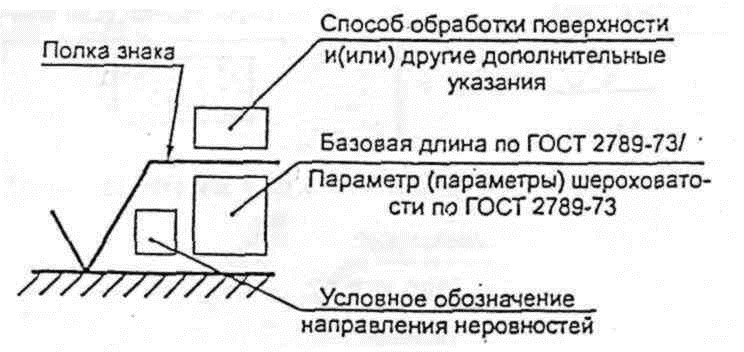
\includegraphics[width=0.6\textwidth]{3sher.png}
		\label{pic:3sher}
		\caption{Обозначение шереховатости}
	\end{figure}
	
	Рабочие (оптические) преломляющие и отражающие поверхности большинства деталей (за исключением, например, матовых стекол, экранов) полируются до высоты неровностей профиля по параметру $R_z$, равному 0,05~мкм.
	
	Нерабочие поверхности могут иметь различные значения параметров шероховатости, зависящие от их назначения, свойств материалов деталей, методов их получения и обработки (литье, прессование, штамповка, резание, шлифование, полировка, травление), характеристик и зернистости обрабатывающего инструмента (абразива). Наиболее часто шероховатость таких поверхностей, достигаемая удалением слоя материала, нормируется параметром $R_a$, равным 2,5 мкм.
	
	В случаях, когда материал детали (например, бериллий, карбид кремния, титановые и алюминиевые сплавы, из которых часто изготовляют зеркала космических телескопов) не позволяет получить оптической поверхности, на нее наносят конструкционное покрытие (стеклянное, медное, никелевое), которое затем обрабатывают (полировкой, алмазным точением) для получения требуемых шероховатости и точности формы поверхности.
	
	Заметим, что оптические поверхности деталей, работающие с мощным лазерным излучением, обрабатываются с применением методов глубокого шлифования и полировки для повышения их лучевой прочности.
	
	\item Допуски на толщину (размер) оптических деталей по (вдоль) оси пучка лучей (линз, пластин, клиньев) устанавливаются обычно симметричными ($\pm$), дающими большую свободу действий оптику, по сравнению с односторонним полем допуска, так как кроме толщины детали он должен выдержать также допуск (более строгий) на точность формы рабочих поверхностей ($N$,  $\Delta N$).
	\item На силовую деталь (линзу, зеркало) устанавливают допустимое значение ее децентрировки. Под \textsc{децентрировкой} понимают смещение центра(ов) кривизны ее рабочей поверхности с базовой оси детали или неперпендикулярность ее плоской рабочей поверхности к этой оси. Силовые детали (линзы, сферические и асферические зеркала, граданы) осуществляют силовое преобразование оптического излучения.  В ряде случаев (например, для цилиндрических рабочих поверхностей, деталей с некруглыми боковыми поверхностями) под децентрировкой понимают смещение или непараллельность центра кривизны либо оси цилиндра рабочей поверхности относительно базовых поверхностей.
	
	Согласно действующему стандарту (ГОСТ~2.412-81), децентрировка задается следующим образом: позиционным допуском, допуском формы заданной поверхности, перпендикулярностью (биением) плоской поверхности.
	
	Расчет допустимых значений децентрировки осуществляется исходя из допустимых значений вызываемых ею дефектов (смещения изображения, аберраций: комы, дисторсии, поперечного хроматизма) и соответствующих коэффициентов влияний децентрировок поверхностей на эти дефекты.
	\item На кромках оптических деталей, как правило, наносят фаски. Фаски подразделяют на:
	\begin{itemize}
		\item защитные (технологические), служащие для удаления микротрещин и выколок, появившихся в процессе обработки детали, предохраняющие ее от возможных сколов, трещин и разрушений при закреплении и эксплуатации из-за больших напряжений в этих дефектах под действием различных сил, а также для исключения травм персонала при изготовлении и сборке деталей из-за острых кромок и заусенцев;
		\item конструктивные, служащие для удаления излишков стекла или для базирования детали (центрировка, обеспечение воздушных промежутков между деталями) по плоской, П-образной, конической, сферической формам буртика;
		\item для крепления завальцовкой (закаткой), приклеиванием, планками.
	\end{itemize}
	
	Защитные фаски и фаски для крепления завальцовкой нормализованы для круглых оптических деталей. Размер (ширина) фаски зависит от диаметра детали, от того на склеиваемую или несклеиваемую сторону она наносится, а угол наклона фаски зависит от отношения ее диаметра $D$ к радиусу $R$.
	
	Размер защитных фасок на углах и ребрах некруглых оптических деталей (например, призм) устанавливают в зависимости от длины наиболее короткого ребра. Фаски наносят перпендикулярно биссектрисам трехгранных или двухгранных углов.
	
	\item На преломляющие и отражающие рабочие поверхности оптических деталей обычно наносят оптические покрытия -- тонкие пленки различных веществ: металлов, окислов металлов, диэлектриков, полимерных соединений, кремнийорганических соединений.
	
	Оптические покрытия позволяют изменять оптические характеристики деталей, придавать им новые физические и химические свойства. В зависимости от назначения покрытия подразделяются на следующие группы:
	\begin{itemize}
		\item просветляющие, зеркальные светоделительные, поглощающие (они изменяют интенсивность проходящего и отраженного излучения);
		\item фильтрующие, поляризующие, спектроделителъные (изменяющие спектральный состав, состояние поляризации и фазовые характеристики излучения);
		\item электропроводящие и защитные (они предназначены для обогрева деталей временной и постоянной защиты деталей, изготовленных из химически- и влагонестойких оптических материалов, для гидрофобной и фунгицидной защиты деталей, работающих в условиях морского и тропического климата, а также абразивной защиты недостаточно прочных материалов). Условные обозначения видов покрытий на чертежах оптических деталей указываются в соответствии с ГОСТ~2.412-81. 
	\end{itemize}
	
	Покрытия могут быть одно-, двух-, трех- и многослойные. На чертеже оптической детали, на контуре поверхности ставят условное графическое обозначение покрытия, а на поле чертежа, в технических условиях, после условного графического знака типа покрытия указывают сведения о покрытии.
	
\end{enumerate}

\section{Оформление оптических схем}

Оформление оптических схем согласно ГОСТ~2.412-81 должно выполняться в соответствии со следующими требованиями:
\begin{enumerate}
	\item На оптических схемах детали и узлы, как правило, следует располагать по ходу светового луча, идущего от плоскости предметов слева направо. 
	\item Для сложных приборов оптическую схему основной части прибора и оптические схемы узлов прибора, имеющих самостоятельное назначение, допускается  оформлять отдельными чертежами. На основной схеме такие узлы допускается обводить штрихпунктирной линией.
	\item Все движущиеся детали (вращающиеся или перемещающиеся вдоль или перпендикулярно к оптической оси системы) следует изображать в основном рабочем положении. При необходимости другие положения подвижной детали(например, крайние) могут быть показаны штрихпунктирной линией.
	\item На оптической схеме следует указывать:
	\begin{itemize}
		\item апертурные диафрагмы и положения зрачков;
		\item положения фокальных плоскостей, плоскостей изображения или предмета, положение полевой диафрагмы;
		\item источники света (схематически);
		\item приемники лучистой энергии (схематически или условными графическими обозначениями);
		\item основные оптические характеристики системы в зависимости от типа, при необходимости -- с допусками (увеличение, угловое поле, удаление выходного зрачка, относительное отверстие, предел разрешения, коэффициент светопропускания);
		\item mразличные дополнительные сведения, например расстояние от последней поверхности фотообъектива до плоскости изображения, линейное перемещение окуляра на 1 дптр, при необходимости -- типы и размеры фотокатодов и ПЗС-матриц;
		\item диаметры диафрагмы и размеры зрачков, размеры тела накала или иных светящихся элементов источников света;
		\item воздушные промежутки и другие размеры по оптической оси;
		\item размеры, определяющие пределы перемещения или предельные углы поворота подвижных оптических деталей;
		\item размеры, определяющие положение оптической системы относительно механической части прибора, например размер, определяющий положение объектива микроскопа относительно нижнего среза тубуса;
		\item габаритные или сборочные размеры, например длину базы, высоту выноса (при необходимости).
	\end{itemize}
	\item В таблицах на оптической схеме указывают:
	\begin{itemize}
		\item фокусные расстояния и фокальные отрезки отдельных узлов оптической системы, которые помещают в поле чертежа в виде таблицы;
		\item  размеры световых диаметров оптических деталей и соответствующих им стрелок прогиба ($ sag = R^2 - \sqrt{(R^2 - \dfrac{D^2_\text{св}}{4})} $, где $ R $ -- радиус кривизны поверхности, $ D $ -- световой диаметр), а также толщину по оси (для призм -- длину развертки), которые помещают в поле чертежа в виде таблицы; 
		\item спецификацию -- перечень деталей, входящих в состав оптической схемы с указанием позиции(формат спецификации стандартный), формата и номера чертежа, количества и названия деталей; 
		располагается эта таблица над основной надписью оптической схемы.
	\end{itemize}
\end{enumerate}

Пример оформления оптической схемы представлен на рис.~\ref{pic:3OS}. Пример оформления схемы комбинированной принципиальной показан на рис.~\ref{pic:3Comb}.

\begin{figure}[h!]
	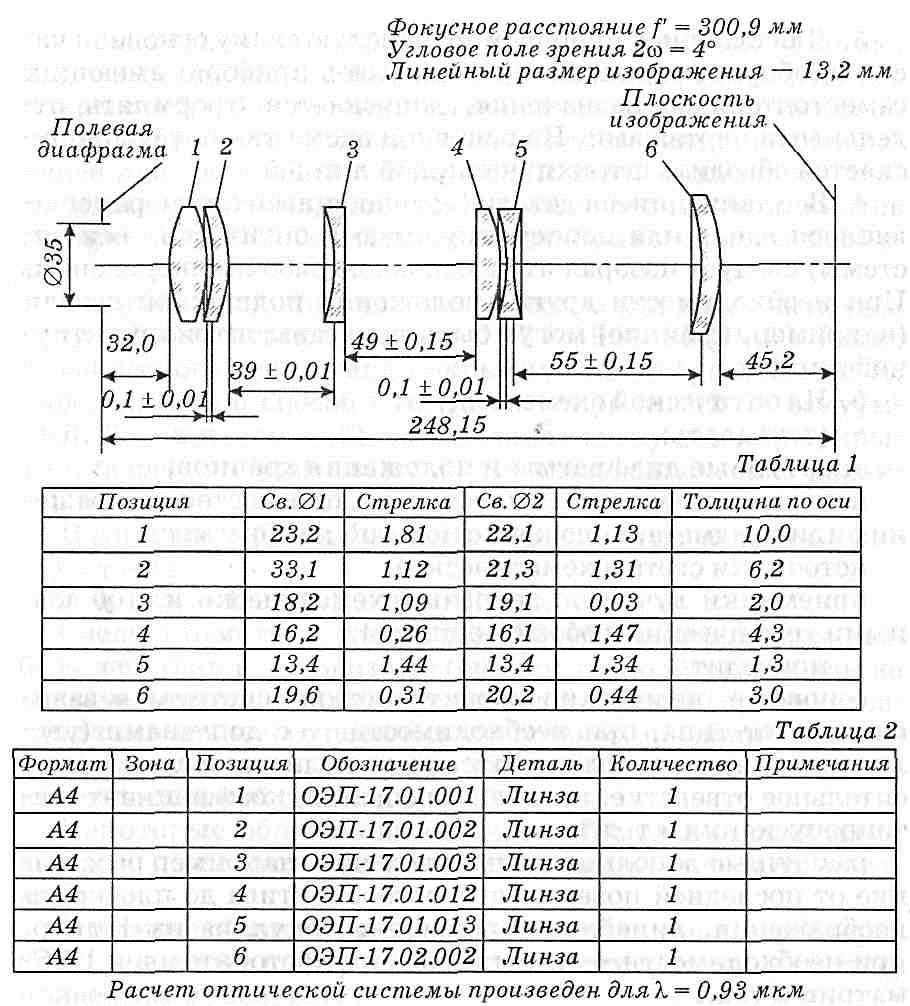
\includegraphics[width=1\textwidth]{3OS.png}
	\label{pic:3OS}
	\caption{Оптическая схема оптико-электронного преобразователя}
\end{figure}

\begin{figure*}[h!]
	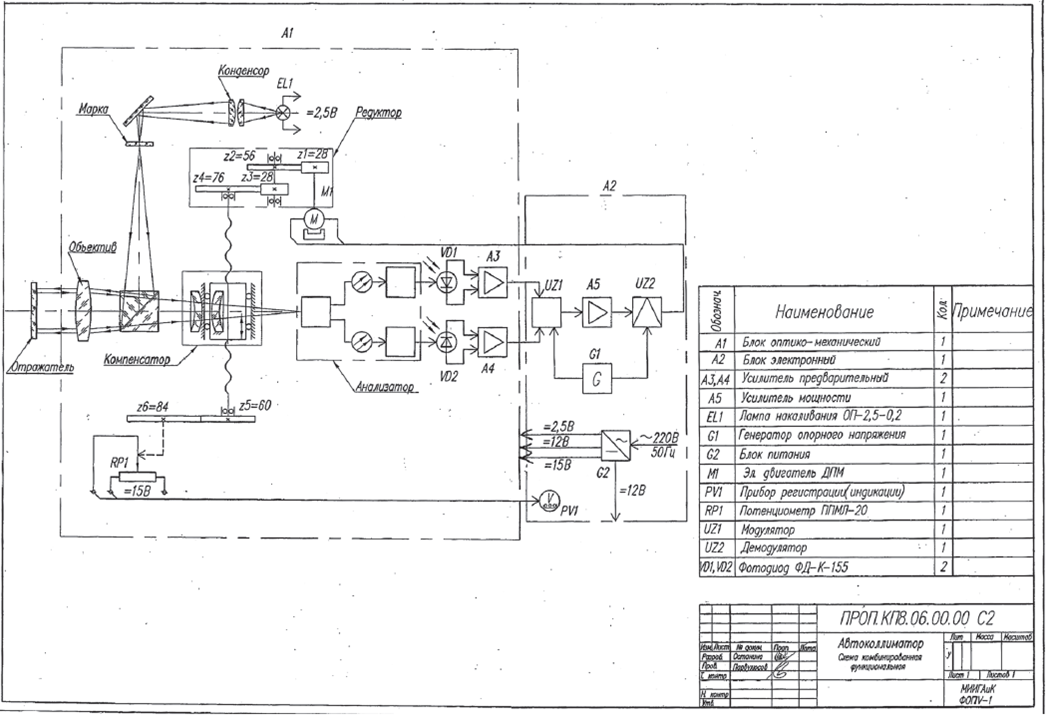
\includegraphics[width=1\textwidth]{3Comb.png}
	\label{pic:3Comb}
	\caption{Схема комбинированная принципиальная}
\end{figure*}